%!TEX root = notes.tex
% Notes from --
% Typed by: Durga

\newpage
\section{Homology and Cohomology}

In this section we briefly review Homology and Cohomology.
Think of it like a crash course on these topics.
For more details you can always refer to \cite{Hatcher2002}. 
As we had discussed before, the Homology and Cohomology are the functors from the category of topological space \(\topsp\) to category of graded abelian group \(\GrAb\) and category of graded ring \(\GrRing\) respectively.

There is two variants of chain complex, one is increasing chain complex and other is decreasing chain complex.
A decreasing chain complex \(C\) of abelian groups is a sequence(or tower) 
\[\dots \xrightarrow{\partial_{i+2}} C_{i+1} \xrightarrow{\partial_{i+1}} C_{i} \xrightarrow{\partial_{i}} C_{i-1} \xrightarrow{f_{i-1}} \dots,\]
where \(C_i\)'s are abelian groups(called chain groups) indexed by integers, and \(\partial_i\)'s are group homomorphisms(called the boundary maps) with \(\partial_{i}\partial_{i+1} = 0, \forall\ i \in \mathbb Z\), in other words,
\[\im(\partial_{i+1}) \subseteq\ker(\partial_{i}).\]
We refer these maps \(\partial\) as boundary maps.
The \(n\)-th homology of a the complex \(C\) is defined as the the quotient
\[H_n(C) = \ker(\partial_n)/\im(\partial_{n-1}).\]
An element of kernel is called a cycle, and that of image is called boundary. 

The increasing chain complex of abelian groups is the same setup as above but the maps points towards the group having higher index.
In increasing chain complex we sometime refer the maps as coboundary maps, and the abelian groups in the complex are called cochain groups.
An element of kernel is sometime called a cocycle, and that of image is called coboundary.
In case of increasing chain complex we sometime call the homology as cohomology.

\begin{definition}[Exact Sequence]
	A sequence of abelian groups \(E\) is called exact if it's homology group \(H_n(E)\) is trivial for all \(n\).
	
	A short exact sequence is an exact sequence of the form 
	\[0 \to A \to B \to C \to 0.\]
	Notice that the map \(A \to B\) is injective and \(B \to C\) is surjective.
\end{definition}
Examples are
\begin{equation}
	\label{nonsplit}
	0 \to \mathbb{Z}/2 \to \mathbb Z/4 \to \mathbb{Z}/2 \to 0,
\end{equation}
\begin{equation}
	\label{split}
	0 \to A \to A \oplus B \to B \to 0.
\end{equation}
Notice that (\ref{nonsplit}) is a short exact sequence but \(\mathbb{Z}/4 \not\cong \mathbb Z/2 \oplus \mathbb{Z}/2\).
The short exact sequence of the form (\ref{split}) is called a split short exact sequence.
The notion of split short exact sequence is completely different in case of non abelian group,	 where a short exact sequence can split in two different ways called left split and right split separately.
We are not going to talk about that in this notes.

\begin{definition}[Chain maps]
	A chain map \(f: A \to B\) between chain complexes \(A\) and \(B\) of same type (i.e., either both increasing or both decreasing) is a collection of maps
	\[f_n: A_n \to B_n \ \forall\ n,\]
	such that following diagram commutes for all \(n\),
	\[\begin{tikzcd} 
		A_n \ar{r}{\partial_n} \ar{d}[swap]{f_n} & A_{n+1} \ar{d}{f_{n+1}} \\ 
		B_n \ar{r}[swap]{\partial_n} & B_{n+1} 
	  \end{tikzcd}\]
\end{definition}
A chain map induces a map in homology 
\[f_\ast: H_\ast(A) \to H_\ast(B).\]

\subsection{Singular Homology and Cohomology}
The \(n\)-simplex \(\Delta^n\) is defined as the following two equivalent ways
\begin{enumerate}
	\item \(\displaystyle \Delta^n \coloneq \left\{(t_0, t_1 \dots, t_n) \mid( 0 \leq t_i \leq 1\ \forall\ i) \land (\sum_{i=0}^n t_i = 1)\right\}\).
	\vspace{1cm}
	
	\begin{description}
		\item[\(\Delta^0\)] \[\begin{tikzpicture}
			%Draw the main axis
			\draw[->] (0,0)--(3,0) node[anchor=west]{X};
			
			%Draw the figure
			\filldraw[red] (2,0) circle (2pt);
			\draw[thick] (1,0.2) -- (1,-0.2);	
		\end{tikzpicture}\]
		\item[\(\Delta^1\)] \[\begin{tikzpicture}
			%Draw the main axes
			\draw[->] (0,0)--(3,0) node[anchor=west]{X};
			\draw[->] (1,-1) -- (1,2) node[anchor=west]{Y};
			
			%Braw the figure
			\draw[thick, red] (1,1) -- (2,0);
			\filldraw[red] (1,1) circle (2pt);
			\filldraw[red] (2,0) circle (2pt);
		\end{tikzpicture}\]
		\item[\(\Delta^2\)] \[\begin{tikzpicture}[3d view={-30}{15}, scale=1]
			
			%Draw the main Axes
			\draw[->] (0,0,0) -- (3,0,0) node[anchor=north east]{X};
			\draw[->] (0,0,0) -- (0,3,0) node[anchor=north west]{Y};
			\draw[->] (0,0,0) -- (0,0,3) node[anchor=south]{Z};
			
			% Draw the figure
			\draw[thick, red, fill=red!20] (2,0,0) -- (0,2,0) -- (0,0,2) -- cycle;
		\end{tikzpicture}\]
	\end{description}
	
	
	\item \(\displaystyle \Delta^n \coloneq \left\{(t_1, \dots t_n) \mid 0 \leq t_n \leq t_{n-1} \leq \dots \leq t_1 \leq 1 \right\}\).
	\vspace{1cm }
	\begin{description}
		\item[\(\Delta^0\)] \[\color{red} \bullet\]
		\item[\(\Delta^1\)]  \[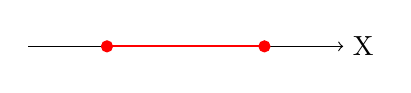
\begin{tikzpicture}
			%Draw the main axis
			\draw[->] (0,0)--(4,0) node[anchor=west]{X};
			
			%Draw the figure
			\filldraw[red] (3,0) circle (2pt);
			\filldraw[red] (1,0) circle (2pt);
			\draw[red, thick] (1,0) -- (3,0);
		\end{tikzpicture}\]
		\item[\(\Delta^2\)] \[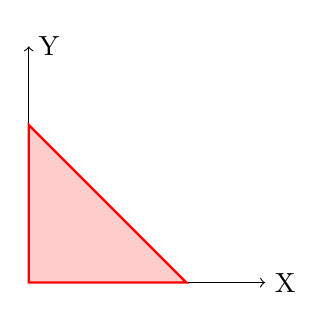
\begin{tikzpicture}
			%Draw the main axes
			\draw[->] (0,0)--(3,0) node[anchor=west]{X};
			\draw[->] (0,0) -- (0,3) node[anchor=west]{Y};
			\draw[thick, red, fill=red!20] (0,0) -- (0,2) -- (2,0) -- cycle;
		\end{tikzpicture}\] 
	\end{description}
	
\end{enumerate}
